\section{Background}
\label{sec:bg}

This section provides relevant background information multi-core memory architectures, and coding theory, and related work.

\subsection{Multi-core Setup and Bank Conflicts}
\label{sec:multi-core}

We consider the generic multi-core architecture illustrated in Figure~\ref{fig:multicore}, where $N$ processor cores rely on a shared memory consisting of $M$ memory banks. All the cores operate in a parallel manner and issue access requests to the shared memory in the event of last level cache misses. These access requests are received by memory controller, which then arbitrates and schedules the requests to be served by different memory banks based on the information stored on the memory banks. In particular, the memory controller maintains different queues for each of the $M$ memory banks, which hold the read and write requests corresponding to the associated bank. These queues are then sequentially served every memory cycle and the acknowledgment with data (in the case of a read requests) is sent to the processor which issued the access request. 

Assuming that the storage space of the shared memory consists of single port memory banks, i.e., it can support a single access request during a memory cycle, multiple access requests issued for content stored on the same bank cannot be served in a single memory cycle. This event is known as a \textit{bank conflict} and leads to increased access latency. The effect of these bank conflicts on the overall access latency of the shared memory becomes even more pronounced as the number of cores increases. Thus, the memory controller needs to avoid such bank conflicts while mapping the access requests from different cores to the memory banks. One straightforward solution to mitigate bank conflicts is to employ multi-port memory banks which can support multiple access requests to the same bank in a single memory cycle~\cite{patterson1997case}. However, the existing designs for multi-port memory banks suffer from increased circuit complexity and large area overhead~\cite{kapasi2003programmable}. Furthermore, in a multi-core setup with large number of cores, it is very likely for a bank to receive multiple simultaneous accesses that can exceed the number of ports present at the bank. Therefore, it's imperative to explore other solutions to the bank conflict problem beyond simply employing multi-port memory banks.

%%%%%%%%%%%%%%%%%%%%%%%%%%%%%%%%%%%%%%%%%%%%%%%%%%%%%%%%%%%%%%%%%%%%%%
%%%%%%%%%%%%%%%%%%%%%%%%%%%%%%%%%%%
%
%%%%%%%%%%%%%%%%%%%%%%%%%%%%%%%%%%%
%%%%%%%%%%%%%%%%%%%%%%%%%%%%%%%%%%%%%%%%%%%%%%%%%%%%%%%%%%%%%%%%%%%%%%
\subsection{Coding Techniques: Preliminaries}
\label{sec:coding_prelims}

Coding theory is the study of various approaches to transform available information into alternative representations with the aim of precisely controlling data redundancy, which enables reliable and efficient processing of the information. Coding has been successfully used in various fields of engineering and computer science, including communications, compression, cryptography, and data storage. The underlying transformation is referred to as a code, and its specific form depends on the application at hand. 

\subsubsection{Block Codes}
\label{sec:block-codes}
In coding theory literature, block codes are one of the most studied classes of codes. An $(n, k)$ block code transforms (encodes) $k$ message symbols belonging to a finite alphabet $\Sigma_1$ to $n$ code symbols belonging to another finite alphabet $\Sigma_2$. In many applications, these finite alphabets are finite fields which are equipped with addition and multiplication operations. The binary set $\{0, 1\}$ with modulo $2$ addition and usual multiplication is an example of a finite field. In addition, we assume that both alphabets are the same finite field $\mathbb{F}$. Under this setup, 
an $(n, k)$ block code encodes vectors in $\mathbb{F}^k$ to vectors in $\mathbb{F}^n$. The vectors in $\mathbb{F}^n$ that are obtained through the encoding process are called {\em codewords}.

The quality of a code is characterized by two parameters: 1) \textit{Rate}, which measures the amount of redundancy introduced during the transformation; and 2) \textit{Minimum distance}, which measures the maximum number of code symbols that can fail without compromising the code's ability to recover the correct message symbols. The rate of a block code is defined as 
$$
\rho = \frac{k}{n}.
$$
The minimum distance of the code $d_{\min}$ is defined as the minimum number of positions at which any two codewords differ. A block code with the minimum distance $d_{\min}$ can allow reconstruction of the original message even after the loss of any $d_{\min} - 1$ codeword symbols~\cite{MacSlo}. Ideally, one would like both the rate and the minimum distance of the underlying code to be as large as possible, however, there is a trade-off between these two parameters~\cite{MacSlo}. Most notably, the Singleton bound dictates that $d_{\min} \leq n-k+1$. Maximum distance separable (MDS) codes attain this bound with equality which makes them optimally resource efficient (as these codes achieve the highest possible rate) for a given failure tolerance. 

Reed-Solomon (RS) codes~\cite{RS1960} are the most celebrated family of MDS codes that exist for all $n$ and $k$. However, these codes typically require working with large field sizes that scale linearly with $n$. That said, we can map the arithmetic over these large fields to the operation of binary field by viewing each element of the large field as a bit vector, e.g., see \cite{shanmugam, GW16}. We will rely on vectorized RS codes in this paper. In contrast to other coding schemes that are employed in existing memory systems like SEC-DED \cite{intel}, BAMBOO \cite{kim}, and ChipKill \cite{ibm}, the RS based memory design in this paper allows for more intelligent memory controller design by improving data access.

\begin{comment}
When available, Reed Solomon codes provide an explicit MDS construction for the pair of parameters $(n,k)$. Often this comes at the expense of a large field size, but in the sequel we describe a method to map the arithmetic to binary operations on the individual bits of each byte vector \cite{shanmugam, GW16}. 
Throughout the design process, adjusting the RS parameters will allow us to achieve other points on the overhead-performance tradeoff. In contrast to other coding schemes for memory systems like SEC-DED \cite{intel}, BAMBOO \cite{kim}, and ChipKill \cite{ibm}, the proposed coding scheme allows for more intelligent memory controller design by improving data access and error correction capability.
\end{comment}

\subsubsection{Encoding Memory Banks}
\label{sec:encoding}

As mentioned above, a coding scheme is characterized by an encoding process that converts message to codewords. In the context of memory banks, we will restrict ourselves to systematic encodings, where message symbols appear as part of the codewords. In particular, we arrange the given information on some memory banks which are referred to as {\em data banks}. Then we generate {\em parity symbols} which are functions of the symbols stored in the data banks and store these parity symbols in new sets of memory banks, referred to as {\em parity banks}. Note that these additional banks, constitute the redundancy in the storage space. Furthermore, in this paper, we only consider encoding across the same row address, i.e., only the content stored on a given row address in the data banks is utilized to generate the parity symbols stored on the same row address in the parity banks.

The following example helps illustrate the key concepts and notation related to encoding memory banks to generate redundant storages space in memory systems. 

 \begin{example}
Consider the setup where information is arranged in two data banks $\mathbf{a}$ and $\mathbf{b}$. Each bank has $L$ rows, each of which can store $W$ bits. Therefore, each bank can be viewed as an $L \times W$ array. For $i \in [L] \triangleq \{1,\ldots, L\}$, let $a(i)$ and $b(i)$ denote the $i$-th row of the banks $\mathbf{a}$ and $\mathbf{b}$, respectively. Moreover, for $i \in [L]$ and $j \in [W] \triangleq \{1,\ldots, W\}$, we use $a_{i, j}$ and $b_{i, j}$ to denote the $j$-th element in the rows $a(i)$ and $b(i)$, respectively. Therefore, for $i \in [L]$,
\begin{align}
a(i) = \big(a_{i,1}, \ldots, a_{i, W}\big) \in \{0, 1\}^W,\nonumber \\
b(i) = \big(b_{i,1}, \ldots, b_{i, W}\big) \in \{0, 1\}^W. \nonumber
\end{align}
Now, given a map $f: \{0, 1\}^W \times \{0, 1\}^W \to \{0, 1\}^W$, we generate a parity bank $\mathbf{p} = f(\mathbf{a}, \mathbf{b})$ such that, for $i \in [L]$, we have
\begin{align}
p(i) = \big(p_{i, 1},\ldots, p_{i,W}\big) = f\big(a(i), b(i)\big).
\end{align}
Among many choices, if we take the function $f$ to be a bit-wise XOR, then we get $\mathbf{p} = \mathbf{a} \oplus \mathbf{b}$, i.e., for $i \in [L]$, 
\begin{align}
p(i) &= \big(p_{i, 1},\ldots, p_{i,W}\big) = a(i) \oplus b(i)\nonumber \\
&\triangleq \big(a_{i,1}\oplus b_{i,1},\ldots, a_{i,W}\oplus b_{i,W}\big). 
\end{align}
Figure~\ref{fig:example1} illustrates this coding scheme. 
%Since the parity bank is based on those rows of the data banks that are indexed by the set $[L'] \subseteq [L]$, we also use the following concise notation to represent the encoding of the parity bank. 
%$$
%\mathbf{p} = \mathbf{a}([L']) +  \mathbf{b}([L']).
%$$
%In general, we can use any subset $\mathcal{S} = \{i_1, i_2,\ldots, i_{L'}\} \subseteq [L]$ comprising $L'$ rows of data banks to generate the parity bank $\mathbf{p}$. In this case, we have
%$$
%\mathbf{p} = \mathbf{a}(\mathcal{S}) +  \mathbf{b}(\mathcal{S}),
%$$ 
%or
%$$
%p(l) = a(i_l) + b(i_l)~\text{for}~l \in [L'].
%$$
%Figure~\ref{fig:example1_case2} illustrates the case with a generic set $\mathcal{S}$.% $ = [L - L'  + 1,\ldots, L]$.
\end{example}

%------------------------------------------------------------
\begin{figure}[t!]
  \centering
  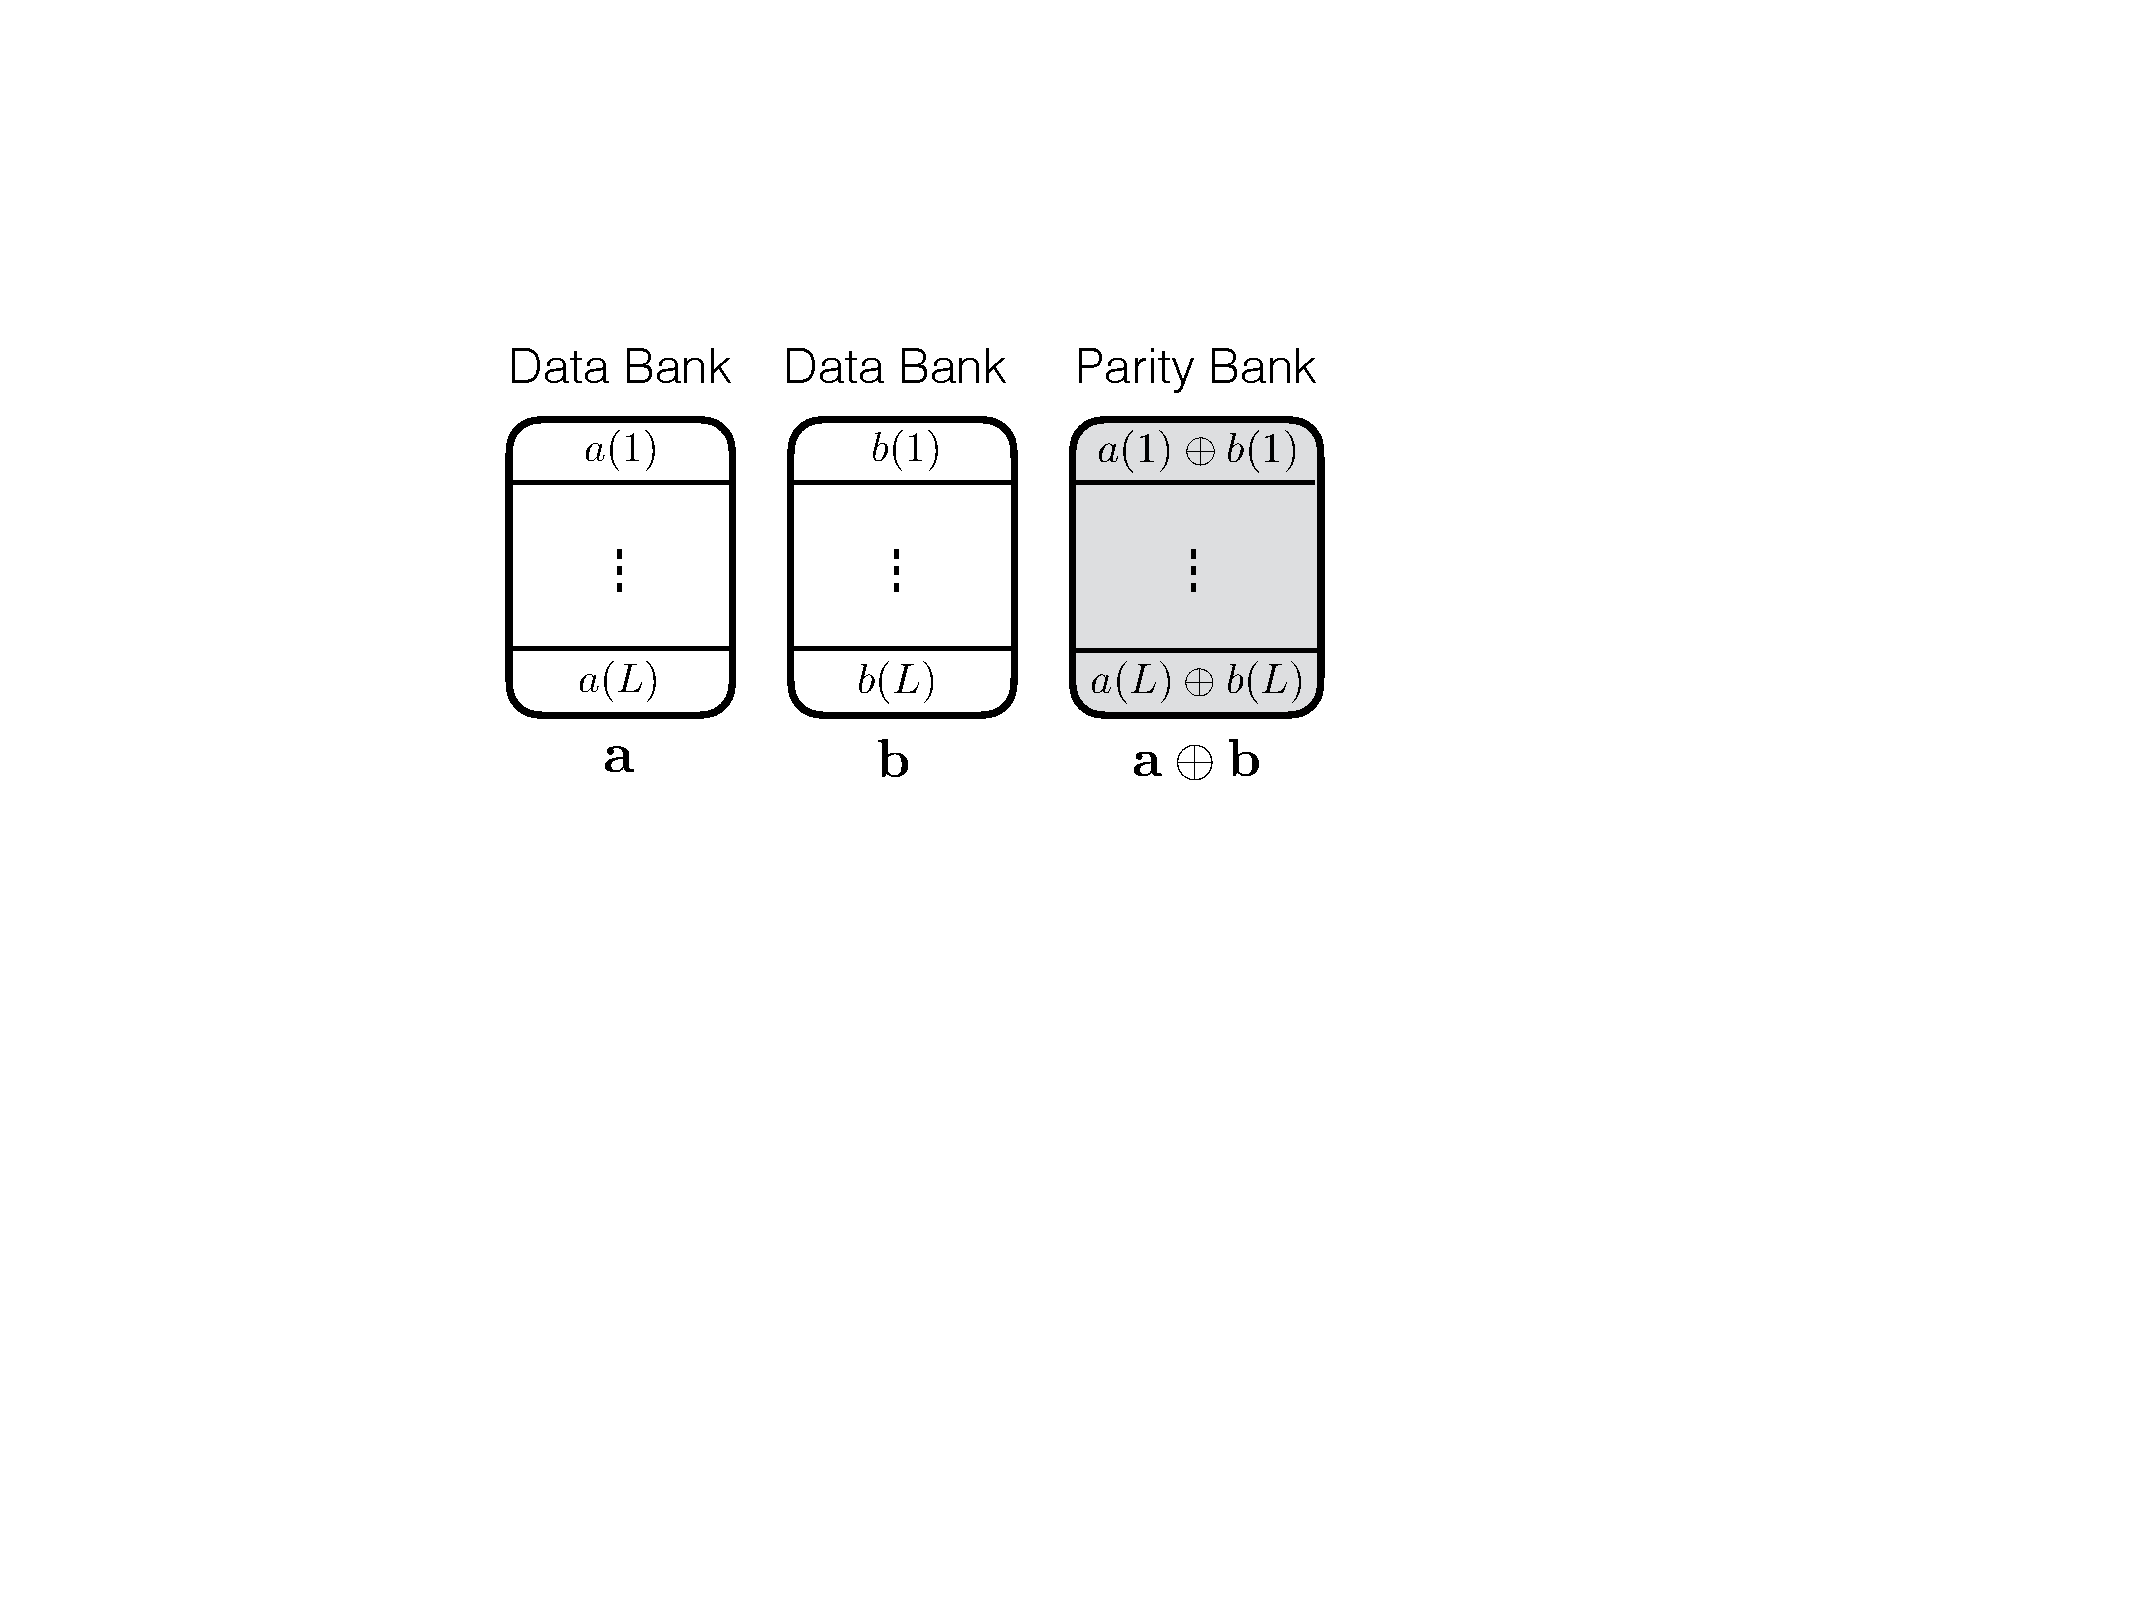
\includegraphics[width=0.65\linewidth]{figures/example-inter-bank.pdf} 
  \caption{Parity bank obtained by performing bit-wise XOR on the two data banks $\mathbf{a}$ and $\mathbf{b}$.}
  \label{fig:example1}
\end{figure}
%------------------------------------------------------------

\begin{comment}
 {\color{blue}
\begin{remark}
{\color{red} Note that we allow for the data banks and parity banks to have different sizes, i.e., $L \neq L'$. This freedom in memory design can be utilized to reduce the storage overhead of parity banks based on the underlying application. The case when the size of a parity bank is smaller than a data bank, i.e., $L' < L$, we say that the parity bank is a {\em shallow bank}. We note that it's perfectly reasonable to have the provisions for shallow banks, especially in proprietary designs of integrated memories in a system on a chip (SoC).}
\end{remark}
}
\end{comment}
%%%%%%%%%%%%%%%%%%%%%%%%%%%%%%%%%%%%%%%%%%%%%%%%%%%%%%%%%%%%%%%%%%%%%%
%%%%%%%%%%%%%%%%%%%%%%%%%%%%%%%%%%%
%
%%%%%%%%%%%%%%%%%%%%%%%%%%%%%%%%%%%
%%%%%%%%%%%%%%%%%%%%%%%%%%%%%%%%%%%%%%%%%%%%%%%%%%%%%%%%%%%%%%%%%%%%%%
\subsection{Emulating Multi-port Memories}
\label{sec:emulation}
A multi-port memory supports multiple simultaneous accesses to content stored in the same memory bank. As evident, such a memory reduces bank conflicts, where some access requests might get delayed due to a single access request accessing a particular memory bank. Therefore, multi-port memories form an essential component of a high performance multi-core setup. That said, designing true multi-port memory banks incurs large cost both in terms of circuit complexity and memory density as compared to single-port memory banks~\cite{Suzuki,WLCH14}.

This has motivated various research efforts to explore algorithm and/or system level designs to emulate the functionality of a multi-port memory using a collection of single-port memory banks, e.g., see \cite{ACP88, EMY91, RG91,CCES93, Memoir_xor, Memoir_xor_virtual} and references therein. The key idea in most of the work in this direction is to employ single port memory banks to store the content in a redundant manner. As a result, when the memory system encounters concurrent accesses leading to bank conflict in a memory bank, it uses the redundancy in the memory banks to create ways to simultaneously serve these accesses using disjoint groups of memory banks. The design of redundant storage space using single-port memory banks is typically based on two general approaches: 1) replication~\cite{ACP88}; and 2) erasure coding~\cite{RG91, Memoir_xor, Memoir_xor_virtual}. 

We briefly illustrate in Fig.~\ref{fig:emulation} how such emulations of multi-port memories work. In particular, consider a setup where we need to store $2L$ rows of data $\mathbf{a} = [a(1),\ldots, a(L)]^T$ and $\mathbf{b} = [b(1),\ldots, b(L)]^T$. We are given single-port memory banks with each bank having capacity to store $L$ rows of data. In order to simplify the exposition, we ignore the write requests for the moment. Our objective is to emulate a multi-port memory that can support $2$ simultaneous read requests to $\mathbf{a}$ and $\mathbf{b}$. Fig.~\ref{fig:emulation_r} describes a replication-based design to support $2$ simultaneous read accesses. Similarly, Fig.~\ref{fig:emulation_ec} shows how one can generate a parity bank by taking element-wise XOR of two data banks to enable $2$ simultaneous accesses. As it is evident from this example, in order to support the same number of read accesses, the replication-based scheme incurs higher storage cost as it requires more single-port memory banks to emulate a multi-port memory bank. This observation is consistent with similar trends observed in other applications, which usually provide opportunities for sophisticated coding schemes to replace replication schemes~\cite{MacSlo, Weatherspoon:2002}. However, in order to make a coding-based solution viable, especially in the context of memory systems, it is essential to employ coding schemes with low computational complexity.

It is easy to generalize the replication scheme (cf.~Fig.~\ref{fig:emulation_r}) to support $r$ simultaneous read accesses by storing $r$ copies of each data element on $r$ distinct single-port memory banks. Similarly, it is possible to employ more sophisticated coding schemes compared to the one in Fig.~\ref{fig:emulation_ec} to support multiple concurrent read accesses~\cite{batchcodes, RSDG16, WKCB17}. However, in order to translate this approach to a viable solution for a memory system, it is necessary to account for write requests as well. Note that the key challenge in employing a redundant storage space in the presence of write requests is to manage consistency across multiple copies of the data. In addition, one needs to ensure that the stale content, i.e., the content modified by a write request, is not supplied in response to a later read request. 

%--------------------------------------------------------------------
\begin{figure}[t!]
\begin{subfigure}{0.52\linewidth}
  \centering
  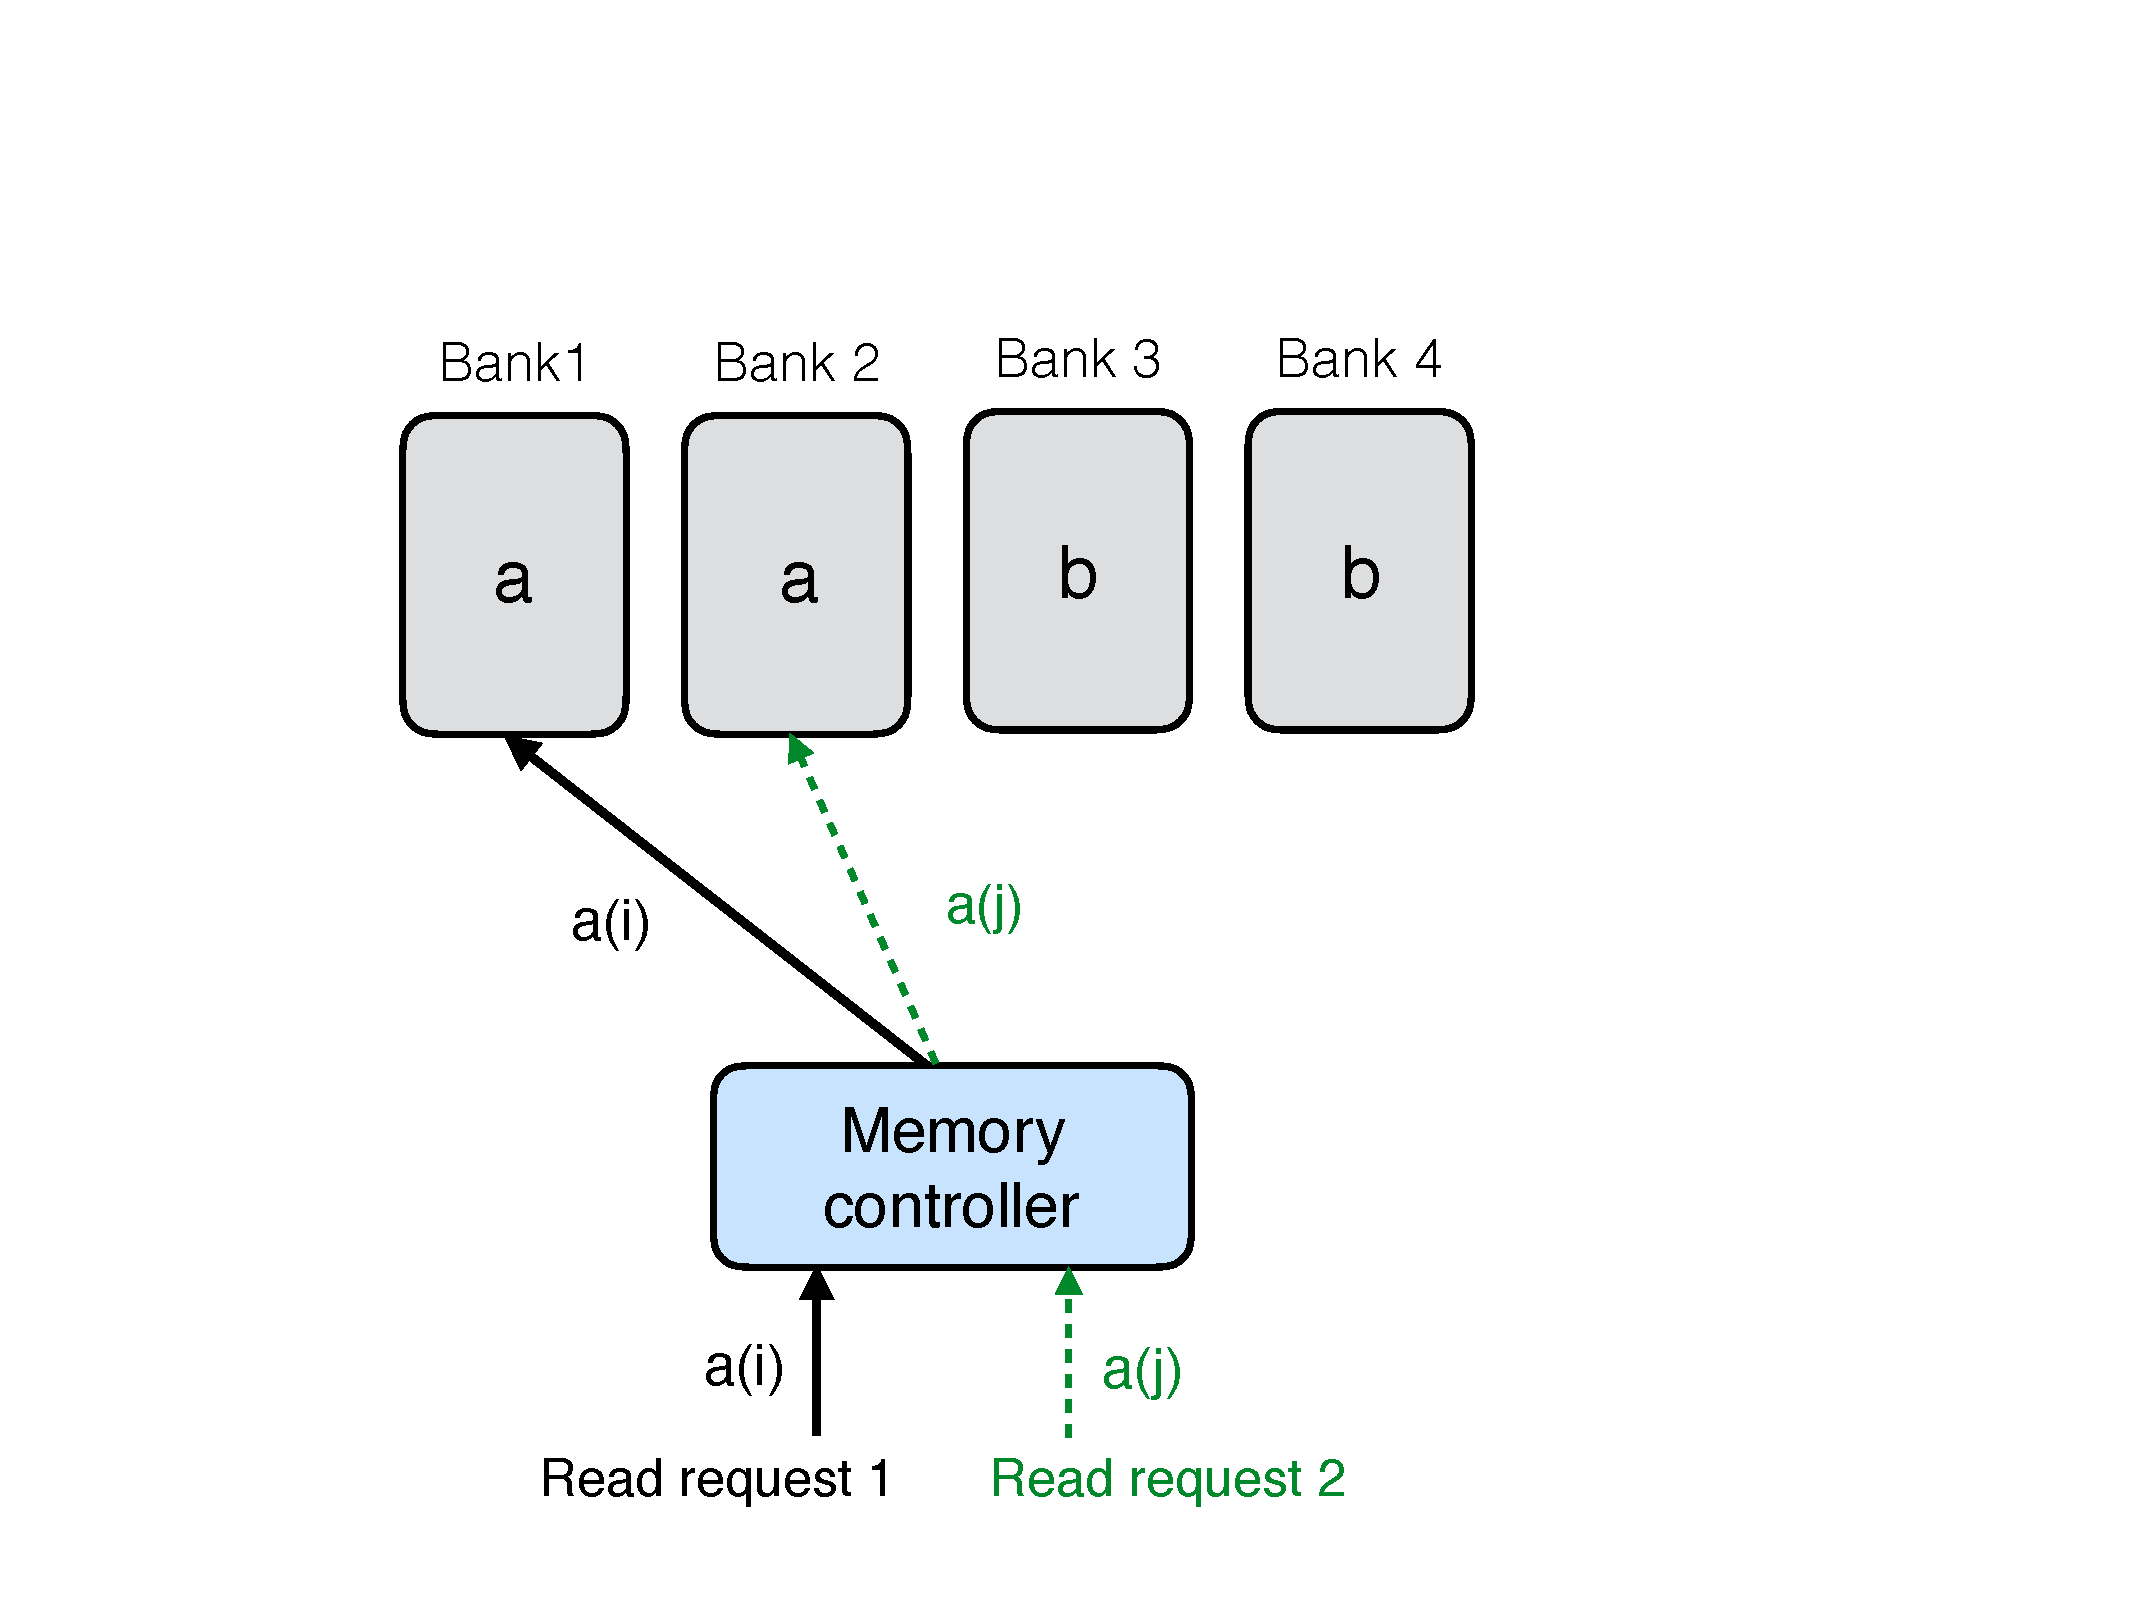
\includegraphics[height=0.92\textwidth]{figures/read-replication.pdf} 
  \caption{$2$-replication scheme.}
  \label{fig:emulation_r}
\end{subfigure}
\begin{subfigure}{0.43\linewidth}
  \centering
  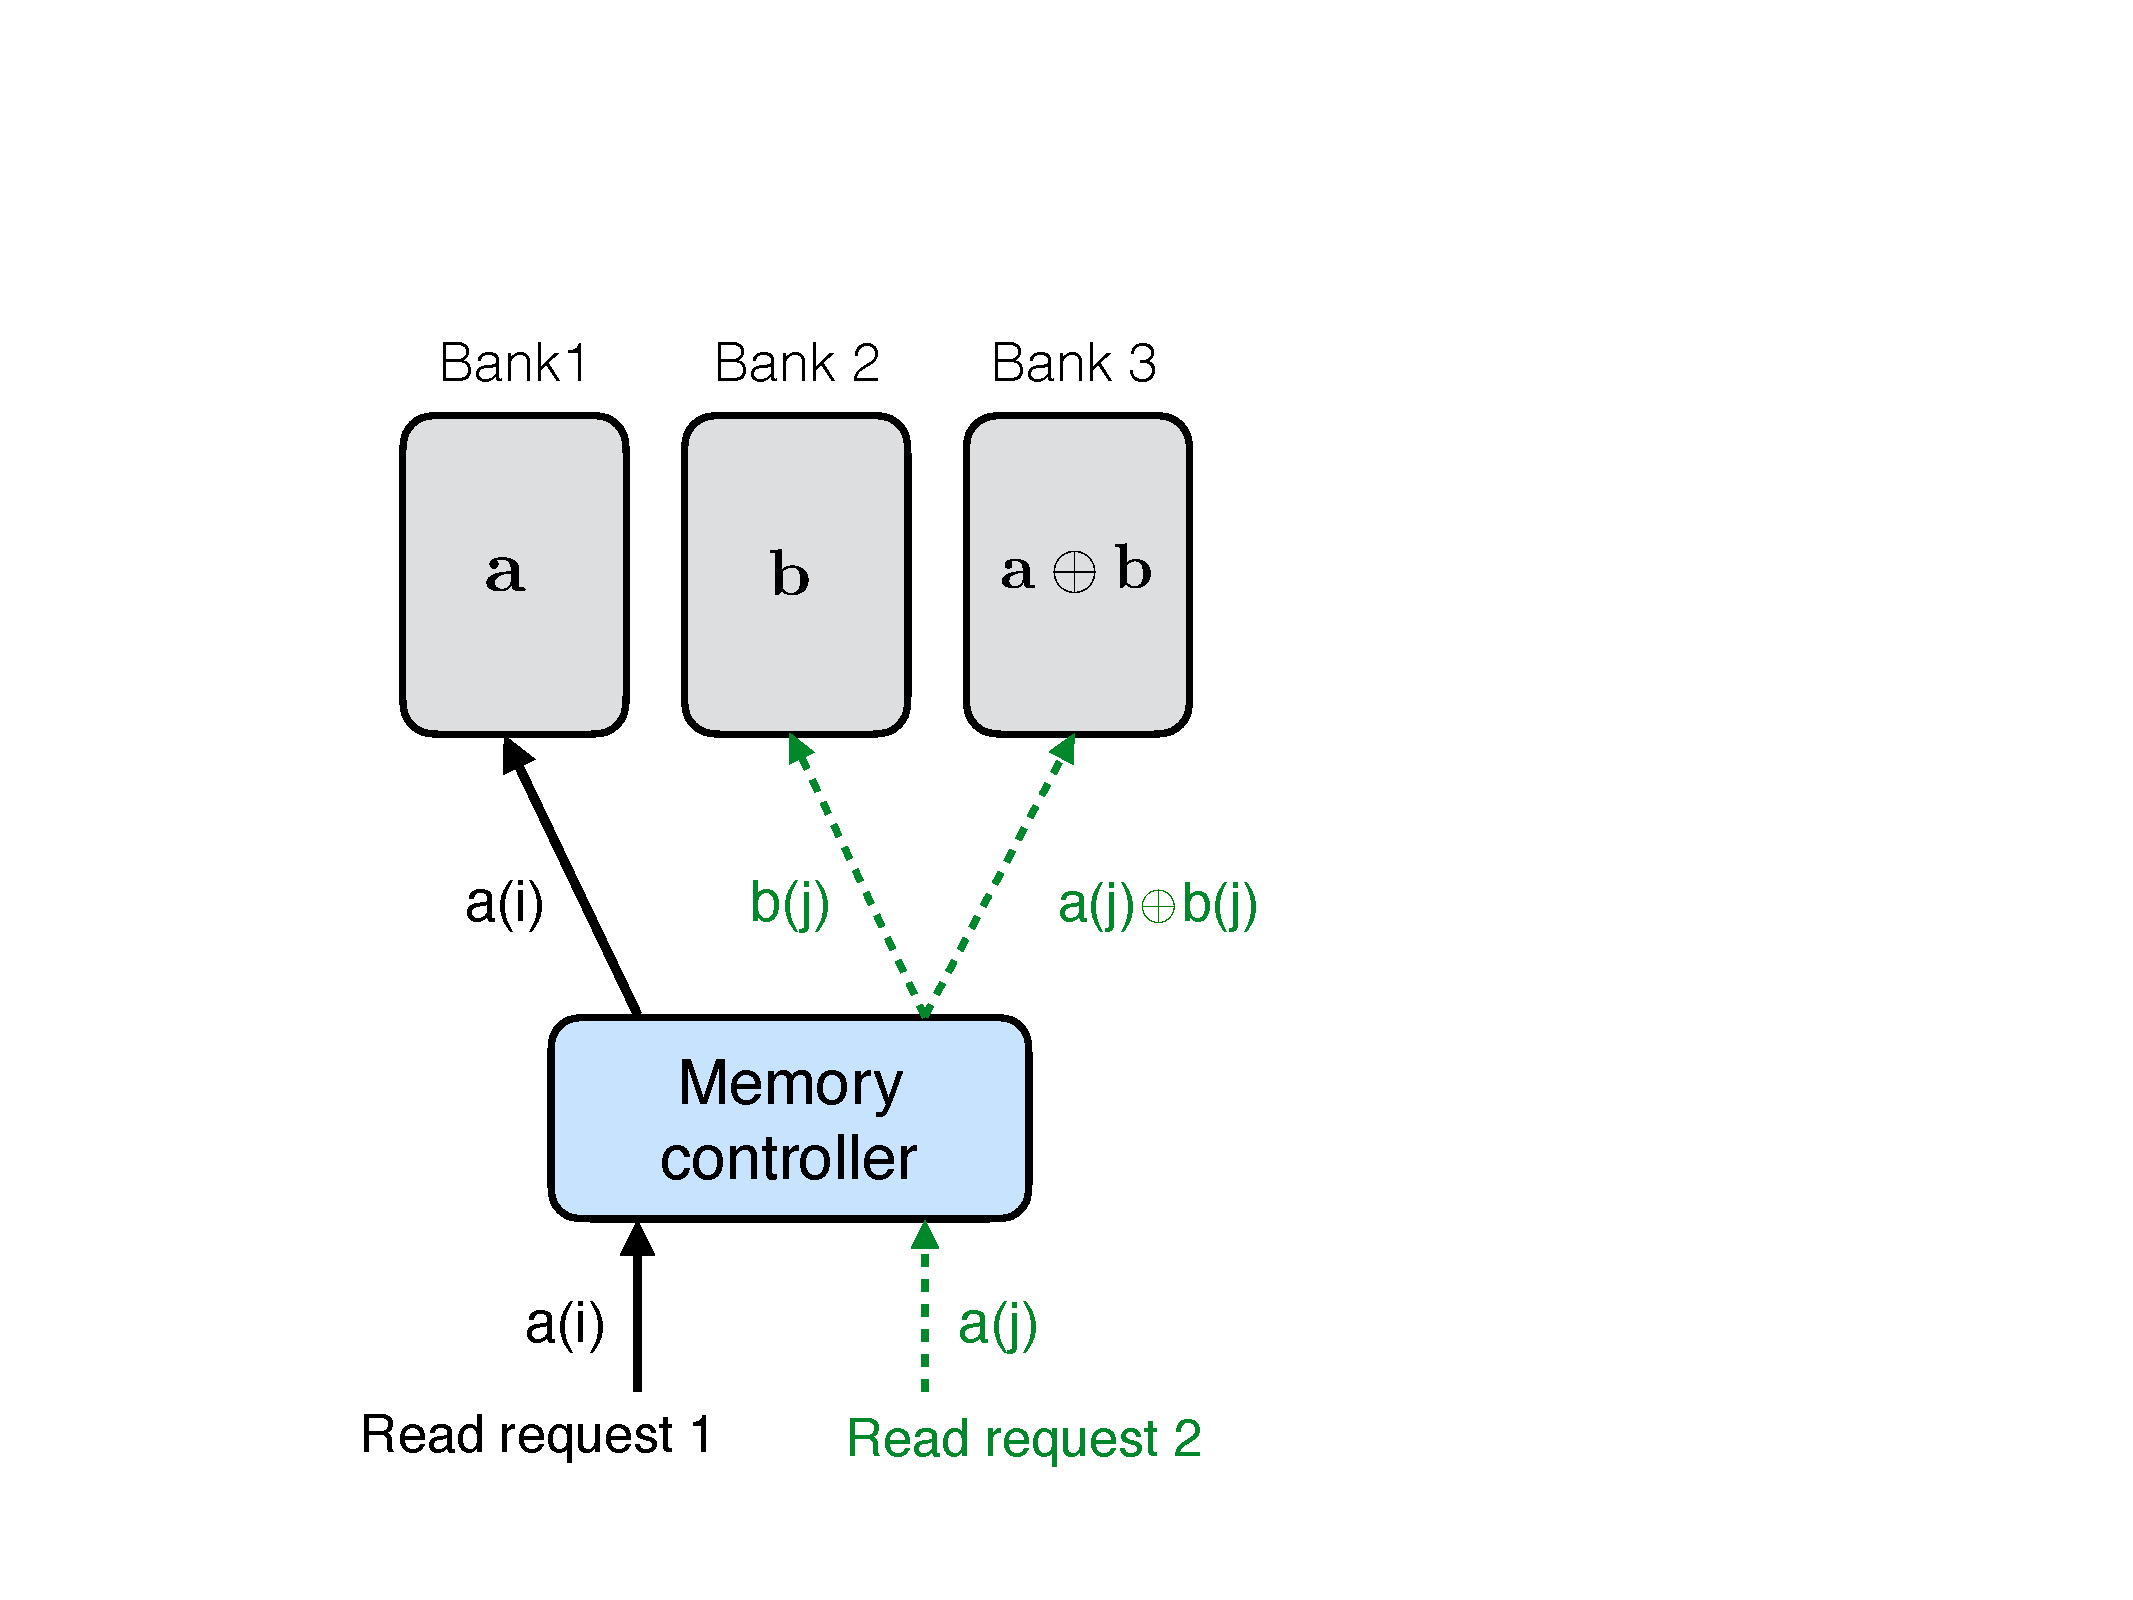
\includegraphics[height=1.1\textwidth]{figures/example-xor.pdf} 
  \caption{Bit-wise XOR.}
  \label{fig:emulation_ec}
\end{subfigure}
\caption{Supporting multiple simultaneous read accesses using single-port memory banks. Let's consider two concurrent requests for data  $\{a(i), a(j)\}$ which cause bank conflict in a single memory banks. 1)  For the replication-based design, since both $a(i)$ and $a(j)$ are stored on $2$ banks, one of those banks can be used to serve each request without causing any bank conflicts. 2) In the coded memory system, as shown in Figure~\ref{fig:emulation_ec}, we can deal with bank conflict in the following manner:  1) First request for $a(i)$ can be directly served by Bank 1, and 2) The read request for $a(j)$ can be served by downloading $b(j)$ and $a(j) + b(j)$ from Bank 2 and Bank 3, respectively.}
\label{fig:emulation}
\end{figure}
%--------------------------------------------------------------------

Towards this, Auerbach et al. demonstrate a replication-based emulation of multi-port memory using single-port memory banks~\cite{ACP88}. This emulation simultaneously supports $r$ read accesses and $w$ write accesses by storing $r\cdot(w + 1)$ copies of each data element on $r\cdot(w+1)$ distinct single-port memory banks. In order to see this, assume that these banks are partitioned in $r$ groups with each group containing $w + 1$ copies of each data element. The $r$ different groups of banks are used to serve $r$ distinct read accesses. Assuming that each group has at least one bank that stores the updated (valid) copy of each data element, we can use that bank to serve the read request from the group. In parallel, for every group, we can perform $w$ write requests on $w$ unused banks in the group. Note that this process does not cause any bank conflicts and all the write requests do get performed inside each group. 

Focusing on coding-based memory designs to support concurrent read accesses, we can modify the ideas from \cite{ACP88} to support write requests as well. We can take set of banks that support $r$ simultaneous read accesses and replicate it $(r+w)$ times~\footnote{We note that depending on the specific coding scheme, one can present a more storage-efficient design. Here, we present a universal scheme that works for any coding scheme.}. Each of these copies is referred to as a \textit{group} of banks. Now, given $r$ read requests we look for the minimum number of groups that store the most updated version of the data elements associated with these read requests and serve all the read requests. In the worst case, this would require using $r$ different groups. For the $w$ write requests, we commit these $w$ requests to $w$ different groups that are not used to serve read requests. Note that there are at least $w$ such groups. While performing a write request inside a group, we update all the memory banks of the group accordingly. 

\begin{remark} Note that the replication-based emulation described above incurs a large overall storage cost as this approach has information rate ${1}/{(r\cdot(w + 1))}$. Moreover, even though the coding-based scheme is storage-efficient in the presence of only read requests, the need to accommodate write requests makes the storage cost of this approach prohibitively large as well. Assuming that the coding scheme has information rate $\rho$, the final rate after $(r + w)$ replications is ${\rho}/{(r + w)}$. In addition to the memory banks, these designs also require additional storage space to store pointers which keep track of which memory banks store the latest versions of the data elements. In order to manage this additional storage requirement, a practical implementation must periodically synchronize every bank with the most recent version of the data.
%{\color{red}In order to keep the storage requirement for maintaining these pointers in check, we need to periodically synchronize all the banks with the most recent version of the data elements.} 
\end{remark}

In the memory architecture proposed in this paper, we completely do away with the additional replications required by the aforementioned emulation approaches to incorporate write requests. In this paper, we instead propose to handle the write requests by modifying the design of the memory controller (cf.~Section~\ref{sec:controller}). This way, we manage to preserve the storage-efficiency of a coding-based solution.

%%%%%%%%%%%%%%%%%%%%%%%%%%%%%%%%%%%%%%%%%%%%%%%%%%%%%%%%%%%%%%%%%%%%%%
%%%%%%%%%%%%%%%%%%%%%%%%%%%%%%%%%%%
%
%%%%%%%%%%%%%%%%%%%%%%%%%%%%%%%%%%%
%%%%%%%%%%%%%%%%%%%%%%%%%%%%%%%%%%%%%%%%%%%%%%%%%%%%%%%%%%%%%%%%%%%%%%

\begin{figure}[t!]
\centering
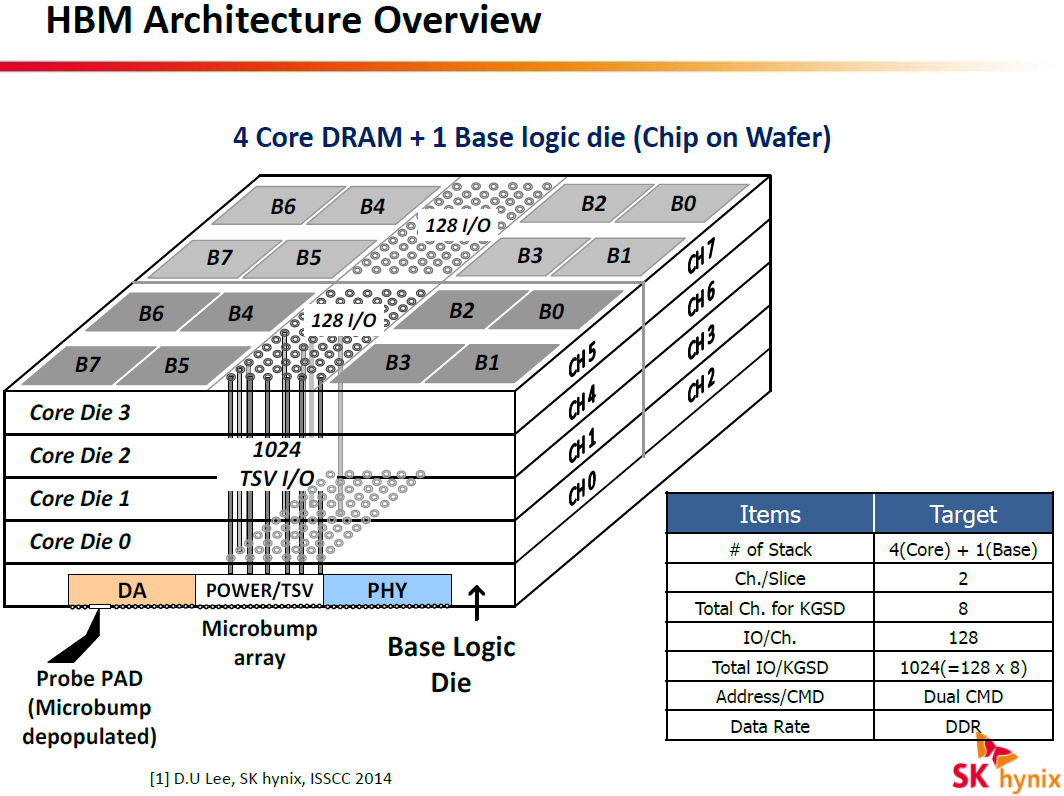
\includegraphics[width=0.99\linewidth]{figures/sk_hynix_hbm_dram_3.jpg} 
\caption{High Density Memory (HBM) architecture\protect\footnotemark. The 3D stacking of memory channels provides an orthogonal plane to pack a large amount of storage in a smaller footprint while maintaining the system's electromagnetic characteristics.}
\label{fig:hbm-arch}
\end{figure}
\footnotetext{Courtesy: \url{http://www.skhynix.com}}


\subsection{High Bandwidth Memory}
\label{sec:hbm}

High bandwidth memory (HBM) standard is defined to enable future high-performance devices such as GPUs. Figure~\ref{fig:hbm-arch} shows a stack of HBM, where it shows $4$ memory core dies vertically integrated together. Each die has $2$ channels, each one with $8$ DRAM banks ($B0$ - $B7$). This memory design enables a 3D scaling of memory, which packs more data in the same space as compared to 2D scaling, while maintaining the I/O signal integrity. The architecture also helps the computing cores to parallelize their access channels, meeting the high data access requirements while consuming less power. Here we only mention the key features of the HBM architecture that are relevant to our goal of reducing access latency using coding techniques. We refer the readers to \cite{kim2014hbm} for a detailed account of various features and specifications of the architecture. 

The key design feature of HBM that allows for parallel access to channels facilitates coded memory storage and retrieval. This enables various storage schemes where both the data and the parity symbols can be stored in the memory banks.


% There are multiple key design parameters in the HBM architecture that facilitates coded memory storage and retrieval. First, the HBM architecture enables ability to access the channels in parallel. This can allow for various storage schemes where the data and codes can be stored. Second, the HBM architecture has a provision where the memory controller can be stored closer to the memory. Additionally, it is also possible to integrate a small logic function next to each bank, which interfaces with the memory controller and performs certain preset arithmetic functions. As shown in Figure~\ref{fig:HBM}, each data bank is now capable of computing codes on the fly by accessing elements from its memory and constructing arithmetic combinations with its locally available logical block. This capability helps the code designers to structure codes which can be constructed dynamically to improve overall efficiency of the system. Local arithmetic also allows designers to draw from similar results and techniques from the field of distributed memory systems for large data servers. Finally, the HBM architecture allows for inter-bank communication, where the data from one back can directly transfer to another bank without going through the main controller. This can allow for optimal reorganization of the memory to improve the access latency. 
%This will enable a distributed memory architecture and thus, will allow for higher optimization of the flow of data and codes between the memory banks and the controller. 
%{\color{blue}Moreover, the ability to have independent channel control for clocks, timing, self refresh, and commands also enhances the capability of a coded architecture. Finally, we also note that HBM architecture provides support for bank grouping, and semi-independent row and column command interface to facilitate activate/pre-charge in parallel with read/writes.} \Ankit{Do we absolutely need the blue colored text? It sounds very vague...If we are not explicitly using these properties in our simulations..we can drop this paragraph.}

%---------------------------
\begin{figure}[t!]
\centering
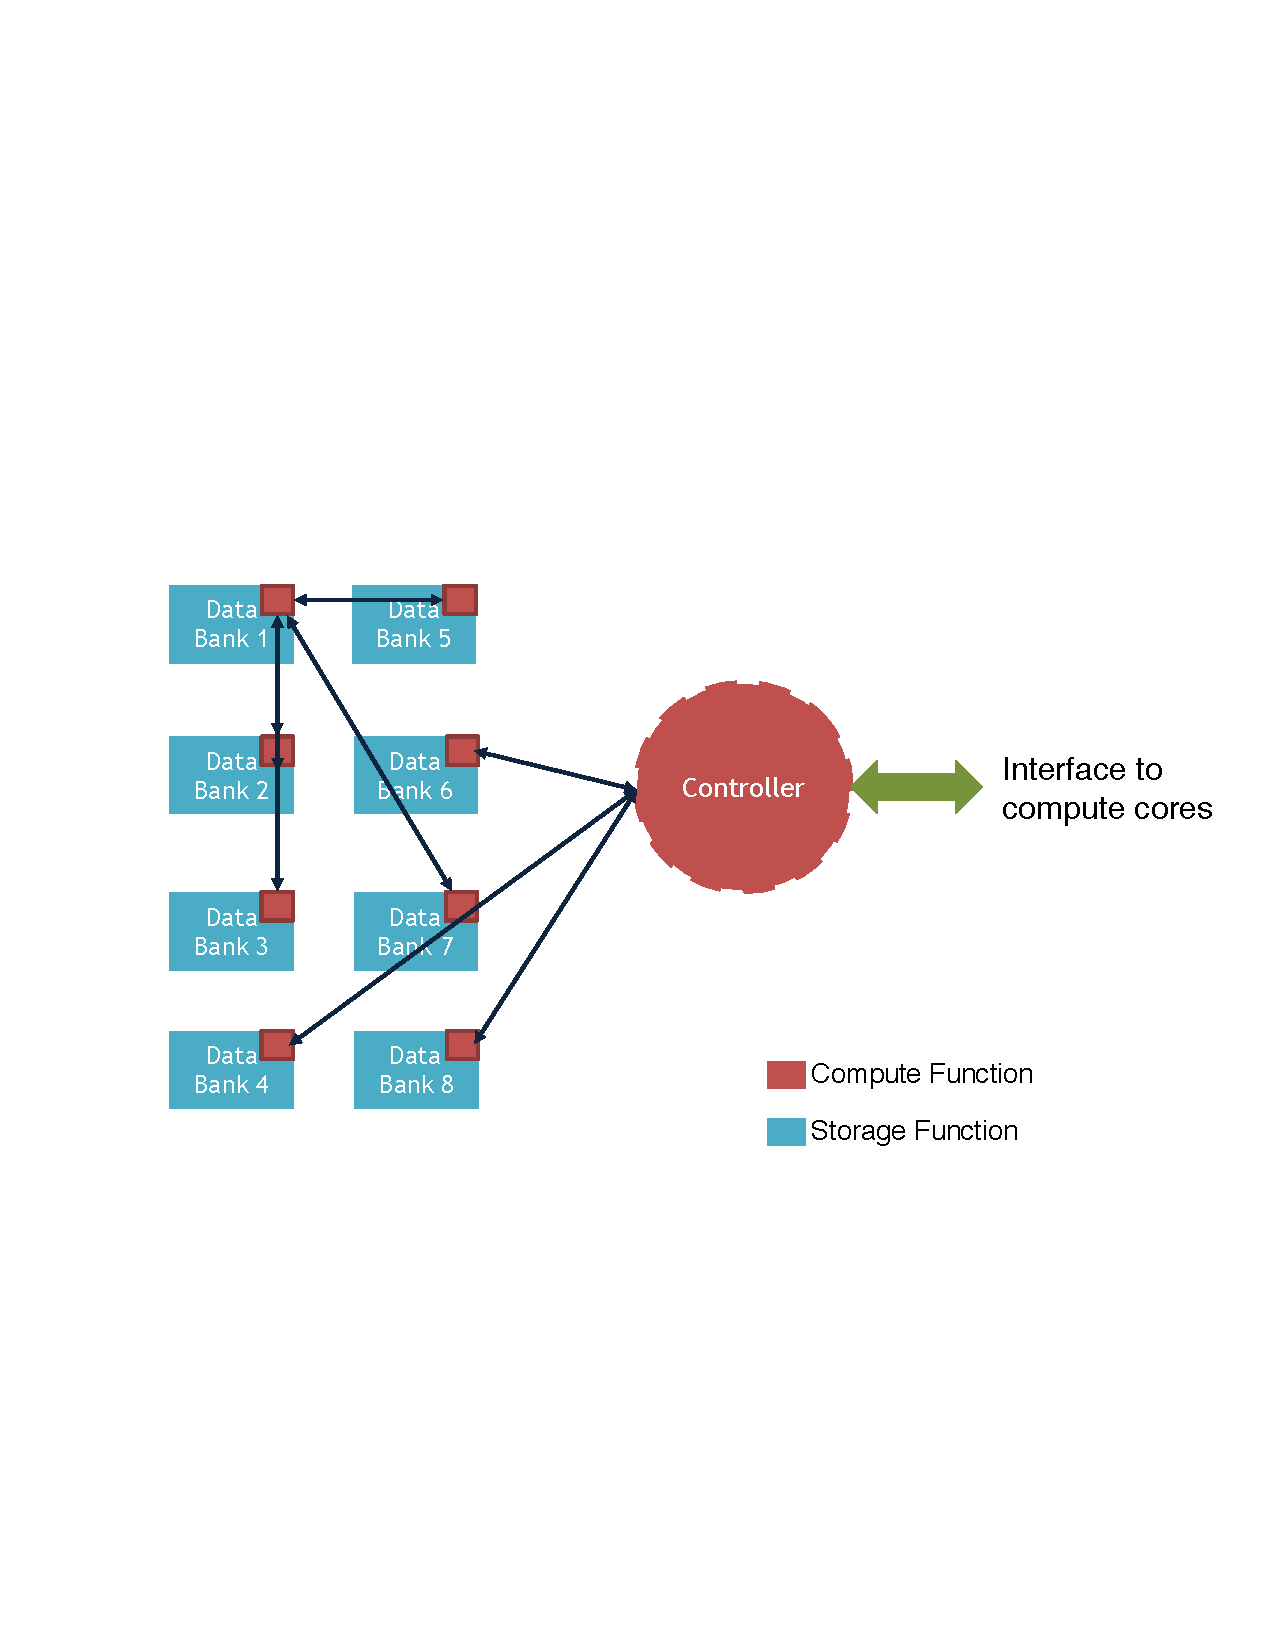
\includegraphics[width=1\linewidth]{figures/New_architecture.pdf}
\caption{Block diagram description of new memory system architectures with distributed memory controllers. This architecture includes a control logic closer to the data bank. This control logic is capable of certain fixed computation that can be exploited to reduce the access bandwidth between the bank and the main controller.%\Ethan{place compute function inside or next to storage function?}
}
\label{fig:HBM}
\end{figure}
%---------------------------

% {\color{red}
% \subsection{Hybrid memory cube}
% \label{sec:hmc}
% \Ethan{remove?}
% A hybrid memory cube (HMC) is a single package containing either four or eight DRAM die and one logic die (Figure 3), all stacked together using through-silicon via (TSV) technology. Within each cube, memory is organized vertically; portions of each memory die are combined with the corresponding portions of the other memory die in the stack. Each grouping of memory partitions is combined with a corresponding controller within the logic die, forming what is referred to as a vault.

% Key features of HMC memory organization:
% \begin{itemize}
% \item Closed-bank memory architecture
% \item Built-in memory controller for each vault
% \item Automatic refresh control over all temperatures
% \item Internal ECC data correction
% \item Advanced RAS features including data scrubbing
% \item Post-assembly repair capability
% \item In-field repair for ultimate reliability
% \item 12.5 Gb/s, 15 Gb/s, 25 Gb/s, 28 Gb/s, or 30 Gb/s SerDes I/O interface
% \item Up to four 16-lane, full-duplex serialized links
% \begin{itemize}
% \item Half-width link (8-lane) and quarter-width link (4-lane) configurations also supported
% \item Up to 320 GB/s effective bandwidth
% \end{itemize}
% \item Packet-based data/command interface
% \item Supports 16, 32, 48, 64, 80, 96, 112, 128, and 256 byte references per request
% \item Error detection (cyclic redundancy check [CRC]) for packets with automatic retry
% \item Power management supported per link
% \item Through-silicon via (TSV) technology
% \item Built-in self-test (BIST)
% \item JTAG interface (IEEE 1149.1-2001, 1149.6)
% \item I2C interface up to 1 MHz
% \item SPI master interface
% \end{itemize}
% }

\begin{remark}
We note that the Hybrid Memory Cube (HMC) architecture~\cite{HMC_slides} is somewhat similar to the HBM architecture discussed here. While our proposed approach could be used in either system, this paper focuses on HBM because it has more publicly available information and data for conducting experiments. The HMC architecture has a provision where the memory controller can be stored closer to the memory. Additionally, it is also possible to integrate a small logic function next to each bank, which interfaces with the memory controller and performs certain preset arithmetic functions. As shown in Figure~\ref{fig:HBM}, each data bank is now capable of computing parity symbols on the fly by accessing elements from its memory and constructing arithmetic combinations with its locally available logical block. This capability helps the code designers to structure codes which can be constructed dynamically to improve overall efficiency of the system. Local arithmetic also allows designers to draw from similar results and techniques from the field of distributed memory systems for large data servers. The HMC architecture also allows for inter-bank communication, where the data from one bank can directly transfer to another bank without going through the main controller. This can allow for optimal reorganization of the memory to improve the access latency. 
%This will enable a distributed memory architecture and thus, will allow for higher optimization of the flow of data and codes between the memory banks and the controller. 
\end{remark}

\newpage

%%%%%%%%%%%%%%%%%%%%%%%%%%%%%%%%%%%%%%%%%%%%%%%%%%%%%%%%%%%%%%%%%%%%%%
%%%%%%%%%%%%%%%%%%%%%%%%%%%%%%%%%%%
%
%%%%%%%%%%%%%%%%%%%%%%%%%%%%%%%%%%%
%%%%%%%%%%%%%%%%%%%%%%%%%%%%%%%%%%%%%%%%%%%%%%%%%%%%%%%%%%%%%%%%%%%%%%
\subsection{Related Work}
\label{sec:related}

\noindent {\bf Coding for distributed storage systems:~}In this paper, we employ coding techniques to store information across multiple memory banks. This is very similar to the application of coding to store data over distributed network of storage nodes in large scale storage systems~\cite{khan, dimakis, Azure12, sathiamoorthy, Hitchhiker}. However, coding for memory systems comes with stringent architectural constraints that need to be taken into account. A memory controller should not be required to perform complex computation during the accesses to the coded information. Moreover, the coding for memory systems also needs to support a significant portion of write requests during memory accesses. Therefore, even though application of coding for improved access latency has been previously explored in distributed storage systems~\cite{batchcodes, RPDV16, RSDG16, WKCB17}, achieving the same goal in the context of memory systems is a challenging problem. 

\noindent{\bf Coding for shared memory:~}In \cite{luan2017dynamic,luan2017intelligent,luan2017intelligent2}, the authors develop a coded data storage architectures which mainly applies to integrated memories in system-on-chip (SoC) subsystems. The proprietary memory design on SoC provides a lot of flexibility to design and implement a complicated coding scheme with less overhead. However, such architectures are limited to a certain subset of products and do not scale to ubiquitous DRAM memories deployed in most computing systems today. The more prevalent DRAM memories are manufactured by multiple vendors and are governed with set industry standards and protocols. Interoperability with commercial devices (and conformity to standards) requires a new design for coded data storage, one which can be implemented by enhancing the memory controller and enables the benefits of a coded architecture. The coding schemes described in \cite{luan2017dynamic,luan2017intelligent,luan2017intelligent2} are suboptimal for the standard memory systems including DRAM and HBM as their specific architectures (cf.~Section~\ref{sec:hbm}) provide the opportunities for further optimization.

In \cite{RG91, Memoir_xor, Memoir_xor_virtual}, the authors also explore coding theoretic techniques in memory systems in order to emulate multi-port memory using single-port memory banks. However, we note that the overall solution proposed in this paper significantly differs from this prior work in both the employed code design and the accompanied memory controller architecture. 

As mentioned earlier, there have been multiple efforts in realizing multi-port memory functionality using various circuit designs (e.g., see \cite{EMY91} and references therein). In this paper we focus on a coding theoretic approach to explore an orthogonal design space. We believe that the previously studied techniques, e.g. pipelined, time-sharing access~\cite{EMY91}, may very well be combined with our coding theoretic framework in order to obtain a more comprehensive solution for high performance memory systems.